\documentclass[14pt]{extreport}
\usepackage{caption}
\usepackage[utf8]{inputenc}
\usepackage[T2A]{fontenc}
\usepackage[english,ukrainian]{babel}
\usepackage{tempora}
\usepackage{float}
\linespread{1.5}
\usepackage{longtable}
\setlength{\parskip}{0pt}
\usepackage{indentfirst}
\usepackage{graphicx}
\usepackage{cmap}
\usepackage{longtable}
\usepackage{titlesec}
\usepackage{geometry}
\usepackage{listings}
\renewcommand{\arraystretch}{1.5}
\geometry{
	a4paper,
	left=20mm,
	right=20mm,
	top=15mm,
	bottom=15mm,
}

\graphicspath{ {./pictures} }
\setlength{\parindent}{4em}

\newcommand\subject{Людино-машинна взаємодія (вбудовані системи)}
\newcommand\lecturer{доцент кафедри ПЗ\\Федорчук Є.Н.}
\newcommand\teacher{доцент кафедри ПЗ\\Федорчук Є.Н.}
\newcommand\mygroup{ПЗ-42}
\newcommand\lab{3}
\newcommand\theme{Моделювання людино-машинної взаємодії (ЛМВ) у ВБ для
моніторингу надзвичайної ситуації}
\newcommand\purpose{Навчитися проектувати інтерфейс з використанням
характеристик людино-машинної взаємодії}

\begin{document}
\begin{normalsize}
	\begin{titlepage}
		\thispagestyle{empty}
		\begin{center}
			\textbf{МІНІСТЕРСТВО ОСВІТИ І НАУКИ УКРАЇНИ\\
				НАЦІОНАЛЬНИЙ УНІВЕРСИТЕТ "ЛЬВІВСЬКА ПОЛІТЕХНІКА"}
		\end{center}
		\begin{flushright}
			\textbf{ІКНІ}\\
			Кафедра \textbf{ПЗ}
		\end{flushright}
		\vspace{20pt}
		\begin{center}
			\textbf{ЗВІТ}\\
			\vspace{10pt}
			до лабораторної роботи № \lab\\
			\textbf{на тему}: <<\textit{\theme}>>\\
			\textbf{з дисципліни}: <<\subject>>
		\end{center}
		\vspace{20pt}
		\begin{flushright}
			
			\textbf{Лектор}:\\
			\lecturer\\
			\vspace{28pt}
			\textbf{Виконав}:\\
			
			студенти групи \mygroup\\
			Коваленко Д.М.\\
			\vspace{28pt}
			\textbf{Прийняв}:\\
			
			\teacher\\
			
			\vspace{28pt}
			«\rule{1cm}{0.15mm}» \rule{1.5cm}{0.15mm} 2025 р.\\
			$\sum$ = \rule{1cm}{0.15mm}……………\\
			
		\end{flushright}
		\vspace{\fill}
		\begin{center}
			\textbf{Львів — 2025}
		\end{center}
	\end{titlepage}
		
	\begin{description}
		\item[Тема.] \theme.
		\item[Мета.] \purpose.
	\end{description}

  \section*{Лабораторне завдання}
  \begin{enumerate}
  	\item Реалізація обчислень розподілу ресурсу транспорту для
парку при заданому ресурсі перевезень пасажирів. Відлагодження для
різних типів транспорту і різних ресурсах перевезень. Обчислення
рішень задачі оптимізації (1) можна проводити в середовищі Ехсеl
  \item Розроблення багатовіконного інтерфейсу з відображенням
кількісного ресурсу для задіяних типів транспорту. Кількість вікон
задається для всіх типів транспорту з його зображенням у окремому вікні
окремого типу , його місткості та обчисленої кількості для типу. Провести
тестування для різних значень ресурсу перевезень пасажирів.
\item Звіт.
  
  \end{enumerate}
  
  \section*{Хід роботи}
  
	
	\begin{figure}[H]
	  \centering
	  \includegraphics[scale=0.7, trim=0 50pt 0 50pt, clip]{1}
	  \caption{Головне вікно програми}
	\end{figure}
	
	\begin{figure}[H]
	  \centering
	  \includegraphics[scale=0.7, trim=0 50pt 0 50pt, clip]{2}
	  \caption{Вікно зображення деталей}
	\end{figure}
	
	\begin{figure}[H]
	  \centering
	  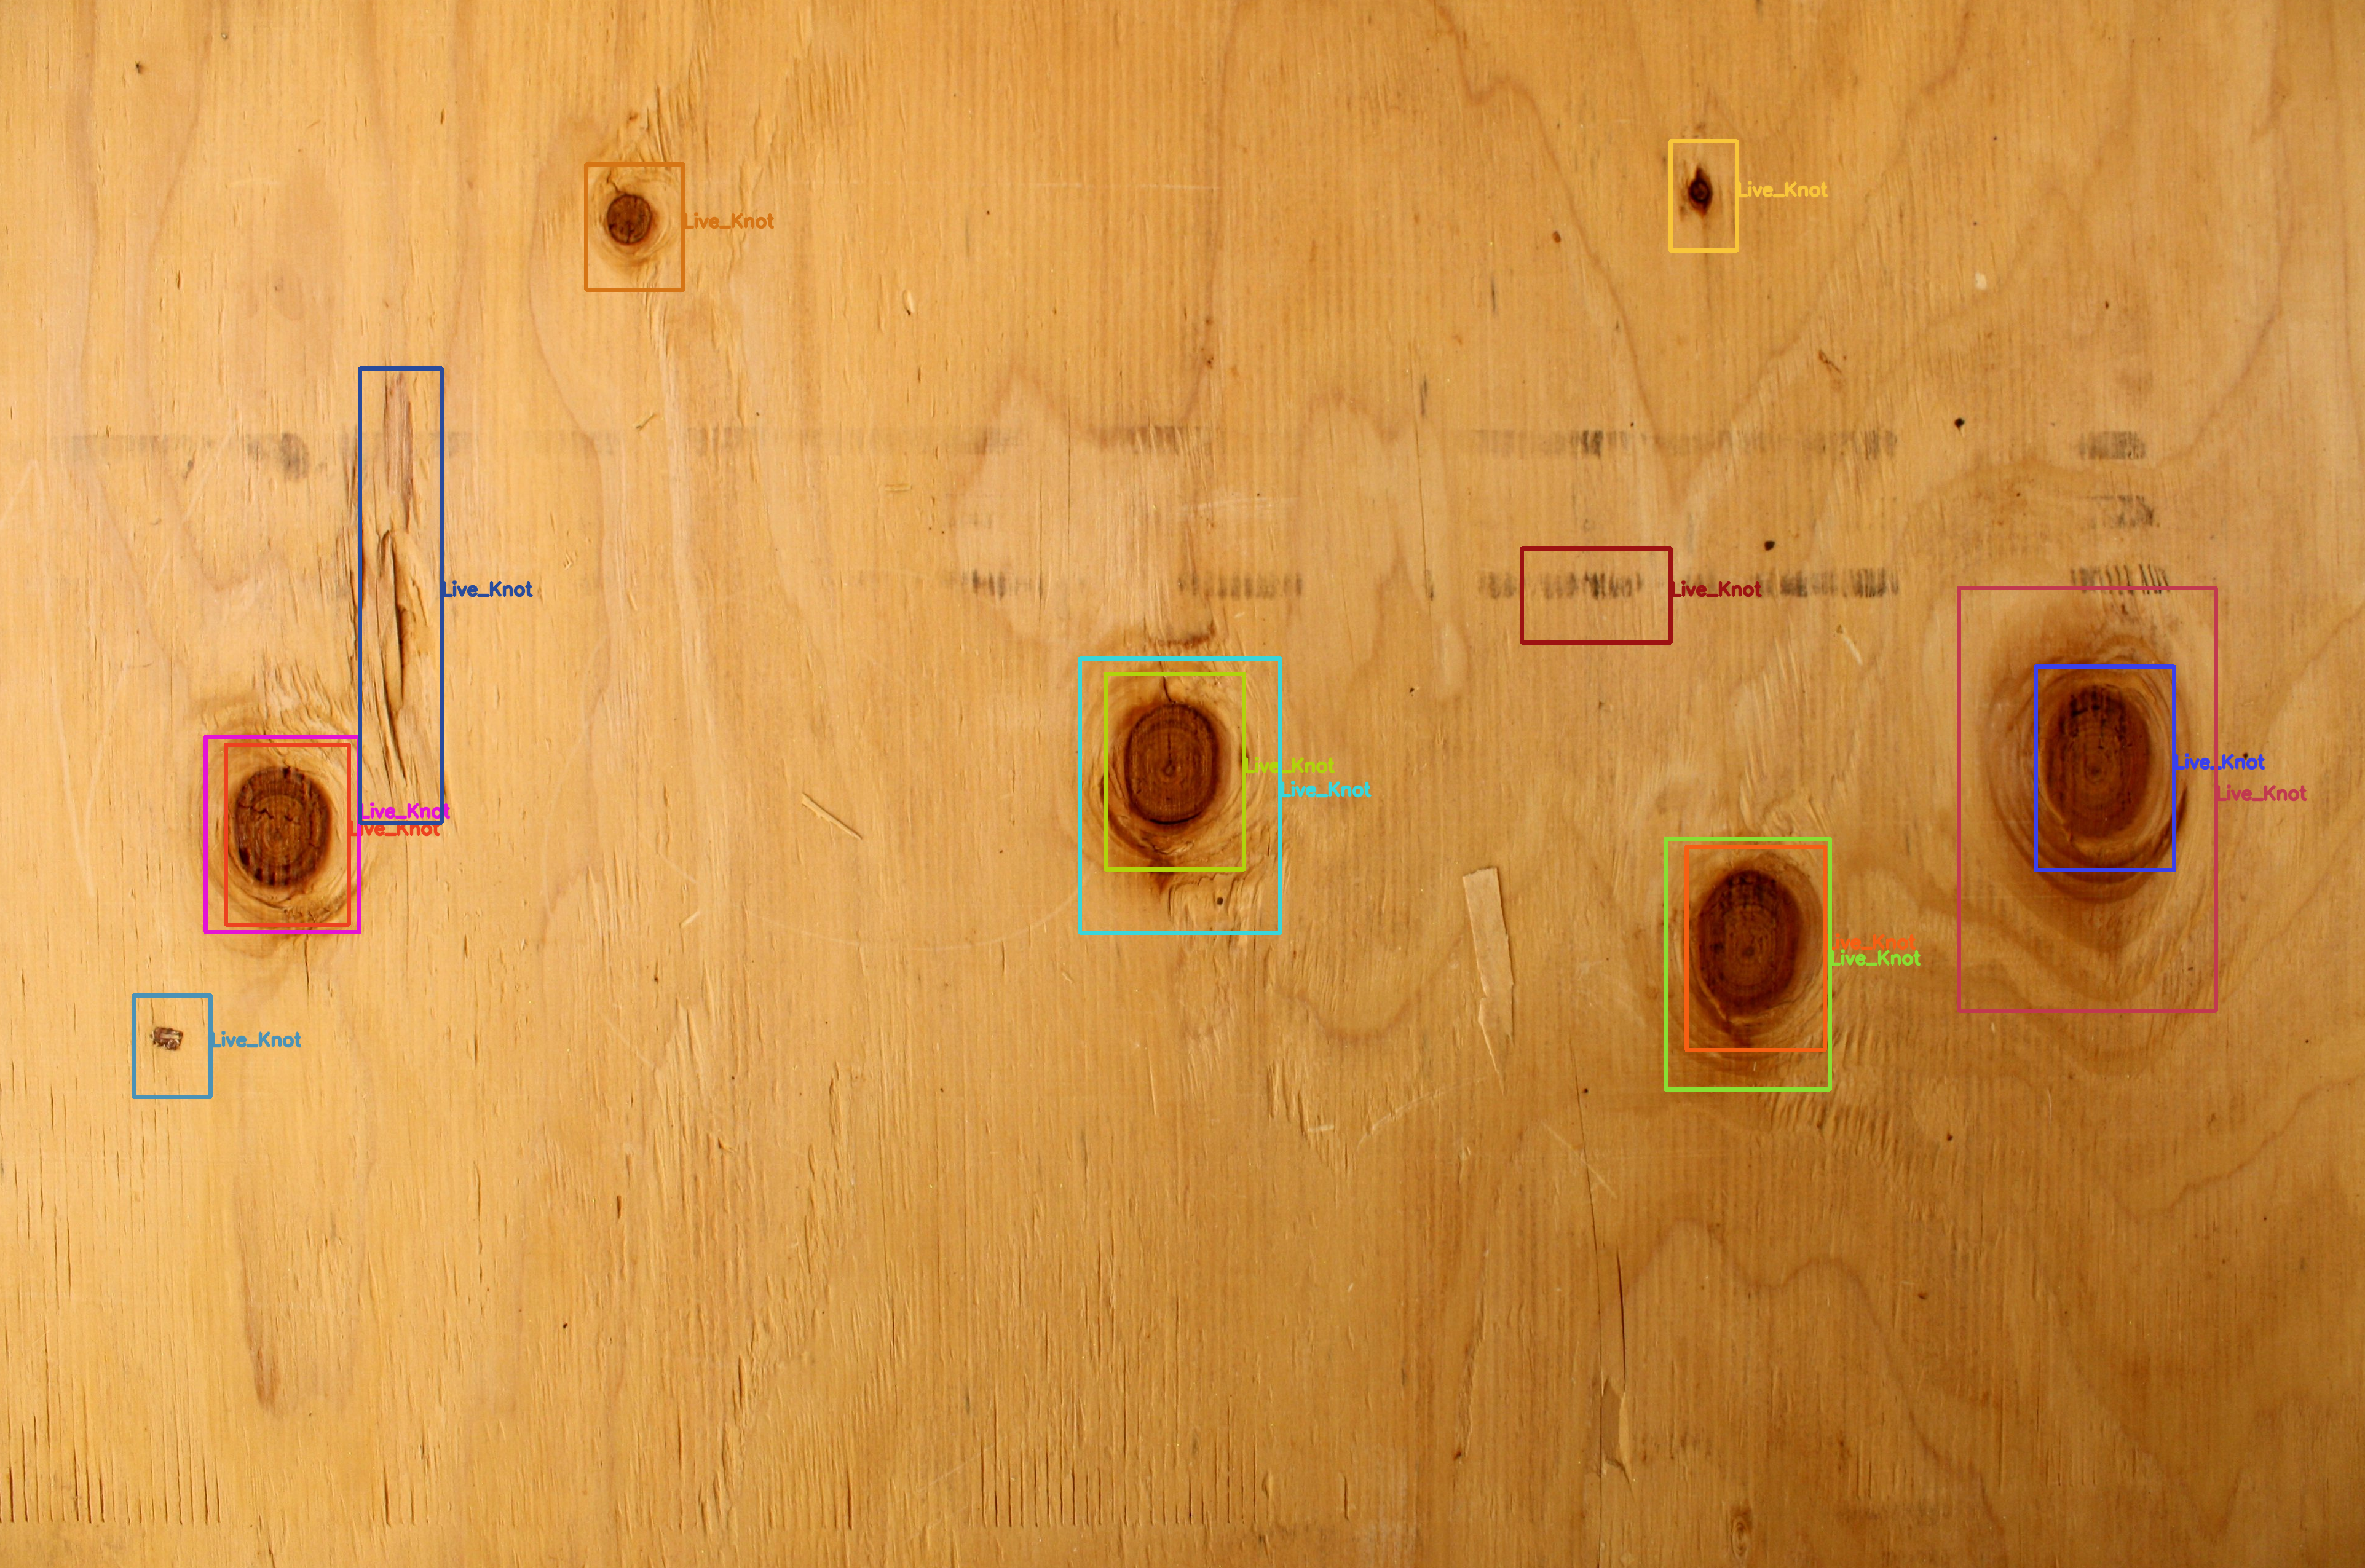
\includegraphics[scale=0.7, trim=0 50pt 0 50pt, clip]{3}
	  \caption{Вікно конфігурації автопарку}
	\end{figure}
	
	\section*{Висновки}
	
Під час даної лабораторної роботи навчився проектувати інтерфейс з
використанням характеристик людино-машинної взаємодії.
	
	    
\end{normalsize}
\end{document}
